\section{Определение инструментов и данных}

Данный раздел описывает инструменты, используемые для программной реализации эксперимента, а
также подготовку данных.

\subsection{Оборудование и программное обеспечение}

Проект реализован на ноутбуке с 16 ГБ оперативной памяти и процессором Intel Core i7 (2,60 ГГц).
Для реализации программной системы выбран язык Python версии 3.9.7, так как данный язык 
программирования предоставляет широкий выбор библиотек для машинного обучения, в частности,
библиотеку scikit-learn. Таким образом, его использование призвано облегчить программную
реализацию алгоритмов машинного обучения и сосредоточиться непосредственно на
эксперименте.

Основные модули, использованные в работе:

\begin{itemize}
    \item[—] Mealpy — библиотека, предоставляющая реализации множества метаэвристических природных алгоритмов;
    \item[—] Nltk — библиотека для символьной и статистической обработки естественного языка для английского языка;
    \item[—] Numpy — библиотека, поддерживающая большие многомерные массивы и матрицы, а также большой набор высокоуровневых математических функций для работы с ними;
    \item[—] Pandas — библиотека для обработки и анализа данных, предлагающая, в частности, структуры данных и операции для управления таблицами и временными рядами;
    \item[—] Scikit-learn — библиотека машинного обучения, включающая в себя различные алгоритмы классификации,
        регрессии и кластеризации.
\end{itemize}

\subsection{Определение наборов данных}\label{datasets}

Для тестирования алгоритмов использовались общедоступные наборы данных, электронные
письма в которых представлены строками.
Список использованных наборов данных:

\begin{itemize}
    \item[—] Набор данных Ling-Spam (2893 писем) \cite{LingSpam};
    \item[—] Набор данных Spam-Assasin (9352 писем) \cite{SpamAssasin};
    \item[—] Набор данных Enron (33715 писем) \cite{Enron}.
\end{itemize}
% TODO здесь еще можно добавить про состав и формат датасетов
С помощью программы, приведенной в Приложении, данные были приведены к единому простому виду, содержащему поля:
содержимое письма (message) и категория (label).

Категория, в свою очередь, может принимать два значения: обычные письма (ham) и спам (spam).

Соотношение спама и обычных писем для набора данных Ling-Spam представлено на \ref{LingSpamScheme},
для Spam-assasin — на \ref{SpamAssasinScheme}, для Enron — на \ref{EnronScheme}.

\begin{figure}[H]
    \centering
    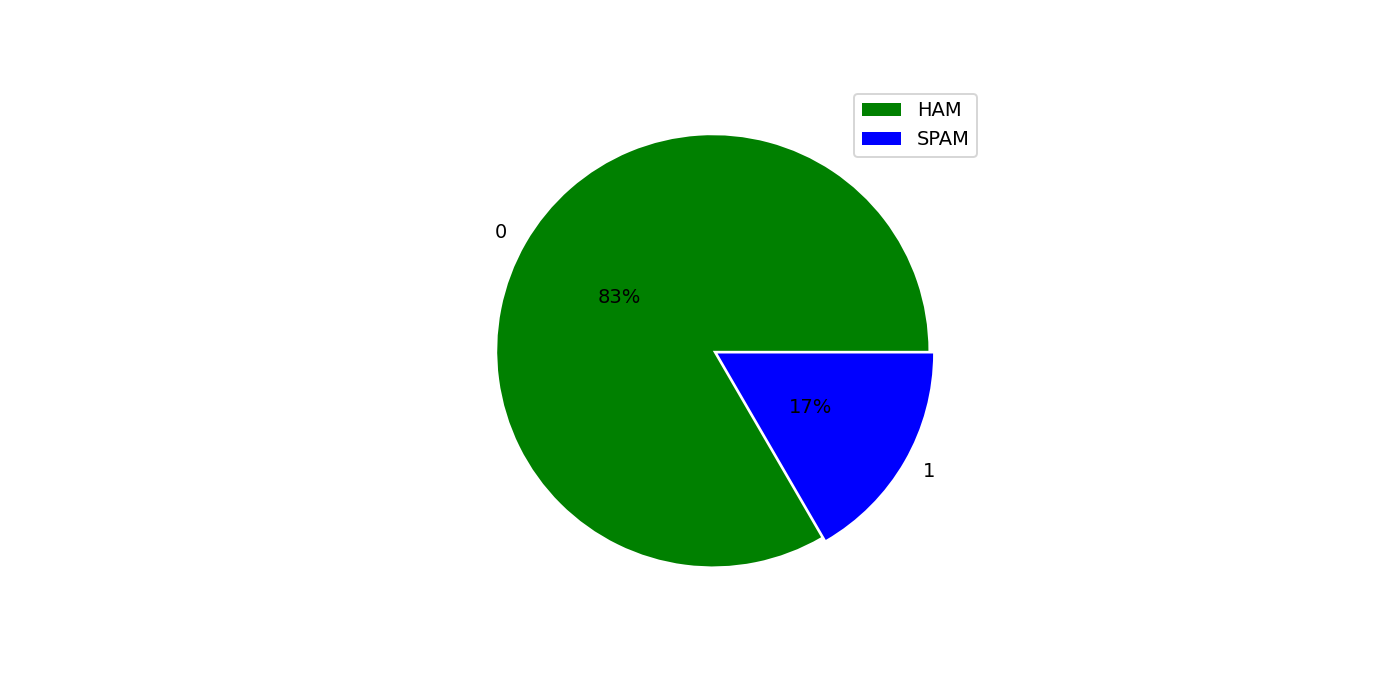
\includegraphics[width=150mm]{static/ling_spam.png}
    \caption{Соотношение спама и обычных писем для набора данных Ling-Spam}
    \label{LingSpamScheme}
\end{figure}

\begin{figure}[H]
    \centering
    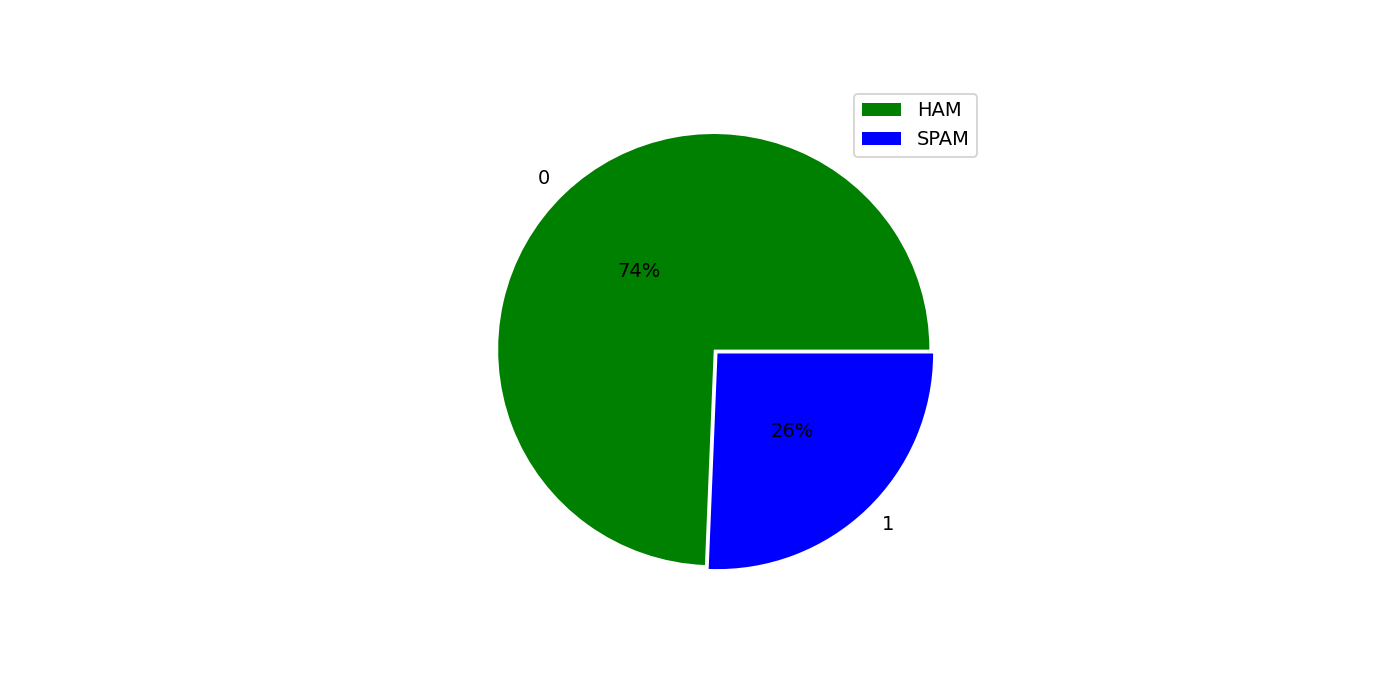
\includegraphics[width=150mm]{static/spam_assasin.png}
    \caption{Соотношение спама и обычных писем для набора данных Spam-Assasin}
    \label{SpamAssasinScheme}
\end{figure}

\begin{figure}[H]
    \centering
    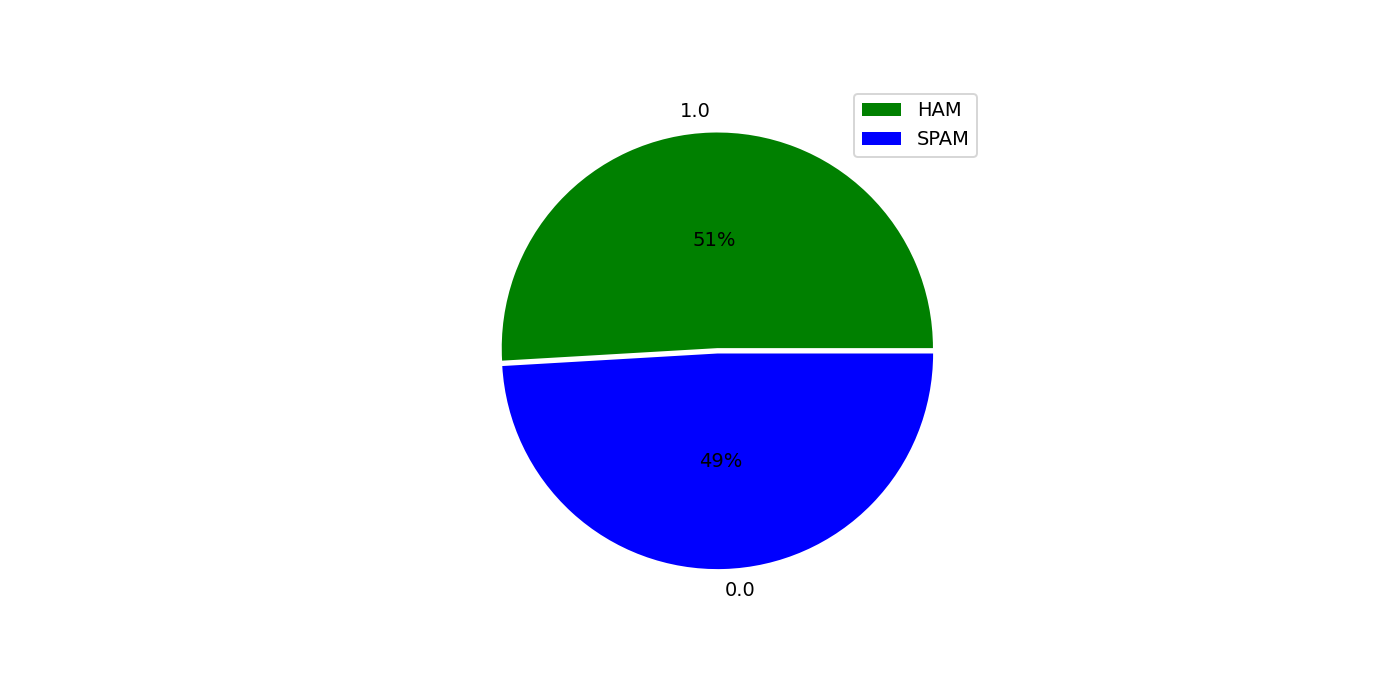
\includegraphics[width=150mm]{static/enron.png}
    \caption{Соотношение спама и обычных писем для набора данных Enron}
    \label{EnronScheme}
\end{figure}


\subsection{Предварительная обработка данных}

Текстовые данные требуют специальной подготовки, прежде чем их можно будет использовать для
моделирования.

Программную реализацию подготовки данных можно найти в \hyperref[App1]{Приложении А}.

\subsubsection{Символьная обработка}

В первую очередь необходимо очистить строки от ненужных символов. Обработка включает в себя:

\begin{itemize}
    \item[—] Замена символов переноса строки и переноса каретки пробелом;
    \item[—] Замена повторяющихся пробелов одним;
    \item[—] Удаление знаков препинания;
    \item[—] Удаление подстрок, не являющихся словами;
    \item[—] Удаление цифр;
    \item[—] Приведение всех букв к строчному виду.
\end{itemize}

\subsubsection{Токенизация}

При работе с текстовыми данными нам необходимо было представить их в виде целых чисел или чисел с плавающей точкой.
Набор текстовых документов преобразовывался в матрицу слов (токенов), из которых состоял текст. При этом нужно было также
исключить из обработки некоторые стоп-слова — различные артикли, предлоги, вводные слова. Это полезно,
поскольку такие слова не очень полезны для определения того, является ли электронное письмо спамом или нет.

Далее матрица подсчета была преобразована в нормализованное представление tf-idf. 
TF-IDF (Term Frequency - Inverse Document Frequency) — это оценка, направленная на определение важности слова
в документе, а также для учета его связи с другими документами из того же набора даннных. Tf (term frequency)
означает частоту слова, а tf-idf — это частота слова, умноженная на величину, обратную частоте,
с которой в наборе данных встречаются документы, его содержащие \cite{Manning}.

Формула, лежащая в основе статистического показателя TF-IDF:
\begin{equation}\label{eq15}
    tf-idf(w, d, D) = tf(w, d) * idf(w, D)
\end{equation}
\\
где:

\begin{itemize}
    \item[—] d — данный документ из нашего набора данных;
    \item[—] D — набор документов;
    \item[—] w — заданное слово в документе.
\end{itemize}

Частота слова среди всех слов документа:
\begin{equation}\label{eq16}
    tf(w, d) = log(1 + f(w, d))
\end{equation}
где $f(w, d)$ — частота слова $w$ в документе $d$.

Обратная частота слова среди всех документов:
\begin{equation}\label{eq17}
    idf(w, D) = log({{N}\over{f(w, D)}})
\end{equation}
где $N$ — количество всех документов в наборе.
